\documentclass[10pt]{article}
\usepackage[T1]{fontenc}
\usepackage{lmodern,amsmath,amssymb,graphicx,hyperref}
\usepackage[margin=.74in]{geometry}
\setlength{\parindent}{0pt}\setlength{\parskip}{7pt}
\begin{document}
\begin{center}{\Large Scalar-only materialized right coefficients}\\[4pt]
Local successor --- 15 November 2026\end{center}
\textbf{Working result.} Draft028 locally elaborates149 theorem statements,
including prior local work, with exit0/no warnings. The printed central
stored-evaluator and actual-entry dependencies use standard foundations.
New results remain outside the Transport53/shared57/fresh project and
outside the original local archive86. All records are unsigned/defaultnot\_covered
[pcc:unverified].

\textbf{Construction without polynomial-representation inputs.}
The new Packed data object contains only a natural scalar denominator and
integer arithmetic-expression syntax. Its rational, variable, arithmetic,
power, sorted-product and geometric constructors do not take polynomial
Rep/Code data as runtime inputs. A separate proof relation matches their
results to the prior actual integer numerator and denominator. This supplies
actual grid, factor, mask, row, denominator and approximation construction without a
favorable expression witness [pcc:unverified].

Normalizer and diagonal scalars also have direct finite-product formulas.
For the actual grid$S$, define
\[
 J(S,t)=\prod_{s\in S\setminus\{t\}}(t-s),\qquad
 \kappa=J(S,0),\qquad \tau_i=-2^i,
\]
\[
 c=\frac{2^{a+1}\kappa^{-1}J(S,\tau_i)}{\tau_i}
     \prod_{j<u}\left(\frac{2^j+2^i}{2^j}\right)^{m_j}.
\]
On the original explicit$i\le a$ domain, these equal the actual normalizer
and diagonal jet. No nodal-polynomial derivative computation is used as a
runtime input to the new construction. Scalar preparation still costs work;
its bit cost is not free or established here [pcc:unverified].

\textbf{Materialized coefficient boxes.} The earlier Box type is a function
on coefficient indices. Value correctness alone does not prevent repeated
child evaluation. The successor uses core
\texttt{Vector (Vector R z) h}: construct each child box, then materialize
the parent with \texttt{Vector.ofFn}. Its view gives exactly the retained
coefficients of full polynomial arithmetic. This establishes value agreement,
not a theorem about compiler behavior, total memory or operation cost
[pcc:unverified].

The actual Packed numerator, trim-zero/noncrossing/scalar branches and finite
extraction agree with canonical actual absolute-right reduction at creation
precision. Existing nonzero signed-grid node,$v_2(t)=i<u\le a$ and bounded-port
premises are retained. Working precision is still$p+E$ for the constructed
denominator exponent$E$, followed by unsigned integer division and odd-part
inversion. The original immutable creation-data/extension-ring interface is
not built here [pcc:unverified].

\textbf{Exact evidence.} Local111 generic payload data6e03ce;
local123 actual scalar products/builders64d18e;
local127 scalar-only entry23543d;
local143 nodes/count model645f3d;
local149 materialized entry1f64e9 (all PCC-20261115- prefixes).
Receipts010--014 retain accepted and failed source/log/exit bytes.
No shared audit/fresh coverage is transferred from parent components.

\newpage
\begin{center}{\Large Actual expression size and count-model boundary}\end{center}
Let$M=\sum_{j<u}m_j$. Logical expression-tree nodes count literals and
operators, including repeated factors. The actual row and denominator
expressions satisfy
\[
 R\le R_*:=17+20\cdot2^a+13M+2u,
 \qquad D\le D_*:=19+10M+2u.
\]
Unary repeated power has exact size$k(N+1)+1$. The cleared geometric
recurrence is bounded by$(N+10)(k+1)^2$. Thus the actual approximation
expression has node bound
\[
 N_*:=1+R_*+(D_*+10)(k+1)^2.
\]
Finite grid cardinality and mask multiplicities are charged. No constant-time
power, free mask witness, shared DAG or fast-power improvement is assumed
[pcc:unverified].

Define a recursive scalar-product MODEL: literals and variables cost0,
addition sums child costs, negation preserves the child cost, and multiplication
adds the coefficient-convolution product count. One convolution has
\[
 P(h,z)=\sum_{b<h}\sum_{n<z}(b+1)(n+1)\le(hz)^2.
\]
The model for the actual approximation is at most$N_*(hz)^2$. This theorem
bounds that declared function. It is NOT yet proved to count operational
execution of the new materialized evaluator. It excludes additions, casts,
array allocation, sorting, scalar/denominator preparation, modular inversion,
integer bit operations and total retained memory. A tested extracted
executable is not supplied [pcc:unverified].

\begin{center}
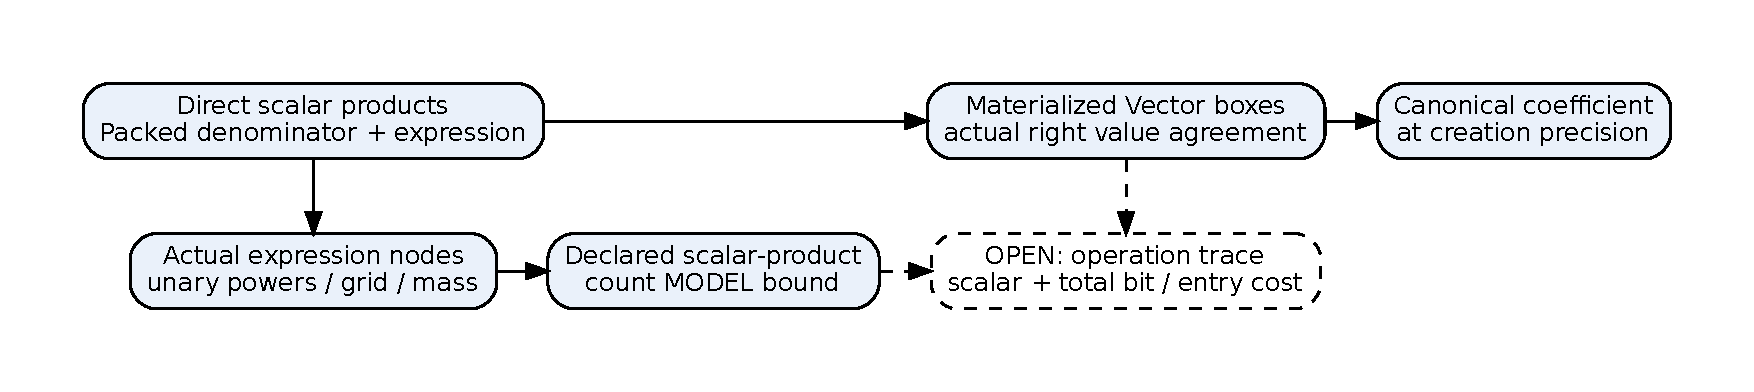
\includegraphics[width=\linewidth,height=1.6in,keepaspectratio]{scalar-dependencies-001.pdf}
\end{center}

\textbf{Next exact obligation.} Add explicit operation events to materialized
Vector evaluation and convolution folds. Prove the value agrees with the
stored evaluator and the event count follows actual loop cardinalities;
attaching the desired recurrence as a counter is insufficient. Then derive
actual literal/scalar sizes and charge rational normalization, enumeration,
sorting, powers, denominator preparation, casts and modular arithmetic in
bits. Every$2^u k$ label remains charged. Original creation, modes, children,
recursion and public expected costs remain separate dependencies
[pcc:unverified].

\textbf{Sources and preservation.} Actual original grid/chart/normalizer/
diagonal/row/right definitions; pinned rational heights and denominators,
finite products/Finset.Sort, and Lean4.35 core Vector Basic/OfFn accessors.
KB unavailable as logged; standard algebra is reused without novelty claims.
Failed020/022/024/025/027 sources and exact raw outputs retained. Original
archive86, Transport151/final16/cost51 and all earlier evidence stay exact.
No native/paid/cloud/attack/timing/scaling campaign was launched
[pcc:unverified].
\end{document}
